\chapter{Flexibility and modularity of GPkit models}

In this section, we will abandon the SimPleAC, and move to examine one of the most sophisticated models and largest models to come out of the CEG, SPaircraft. SPaircraft is a commercial aircraft design tool that makes use of component-based performance modeling to optimize different configurations of aircraft in both single- and multi-mission scenarios. 

\section{Component-based design}

\section{Example problem: Creating a modular tail structural model}

Consider the set of equations considered in \cite{SP_ac_design} to size
the structure of a conventional horizontal tail. 

\begin{align}
    0.92 w\tau_{\rm{ht}} t_{\rm{cap}}^2 + I_{\rm{cap}} &\leq \frac{0.92^2}{2}w\tau_{\rm{ht}}^2t_{\rm{cap}}\\
    8 &\geq N_{\rm{lift}}M_{\rm{r}}(\AR_{\rm{ht}})q_{\rm{ht}}^2\frac{\tau_{\rm{ht}}}{S_{\rm{ht}} I_{\rm{cap}}\sigma_{\rm{max}}}\\
    12 &\geq \frac{L_{\rm{max}} N_{\rm{lift}} q^2}{\tau_{\rm{ht}} S t_{\rm{web}} \sigma_{\rm{max-shear}}}
\end{align}

Now, using a set of variables that includes the original parametrization of the wing, 
we would like to extend this structural model to be able to design a pi horizontal tail
with the same loading. 

This section will derive a new set of constraints, which are compatible with 
both conventional tail and pi-tail architectures, and in the process demonstrate the 
capabilities of \gls{GP} in incremental design. 

\subsection{Thinking about pi-tail loading}

\subsubsection{Sample Free Body Diagram and Load Distributions}
\label{s:loadDistributions}

With the aforementioned assumptions, the free body diagram diagram of the 
pi-tail is shown at the top of Figure~\ref{fig:HTFBD}. 

\begin{figure}[!ht]
\centering
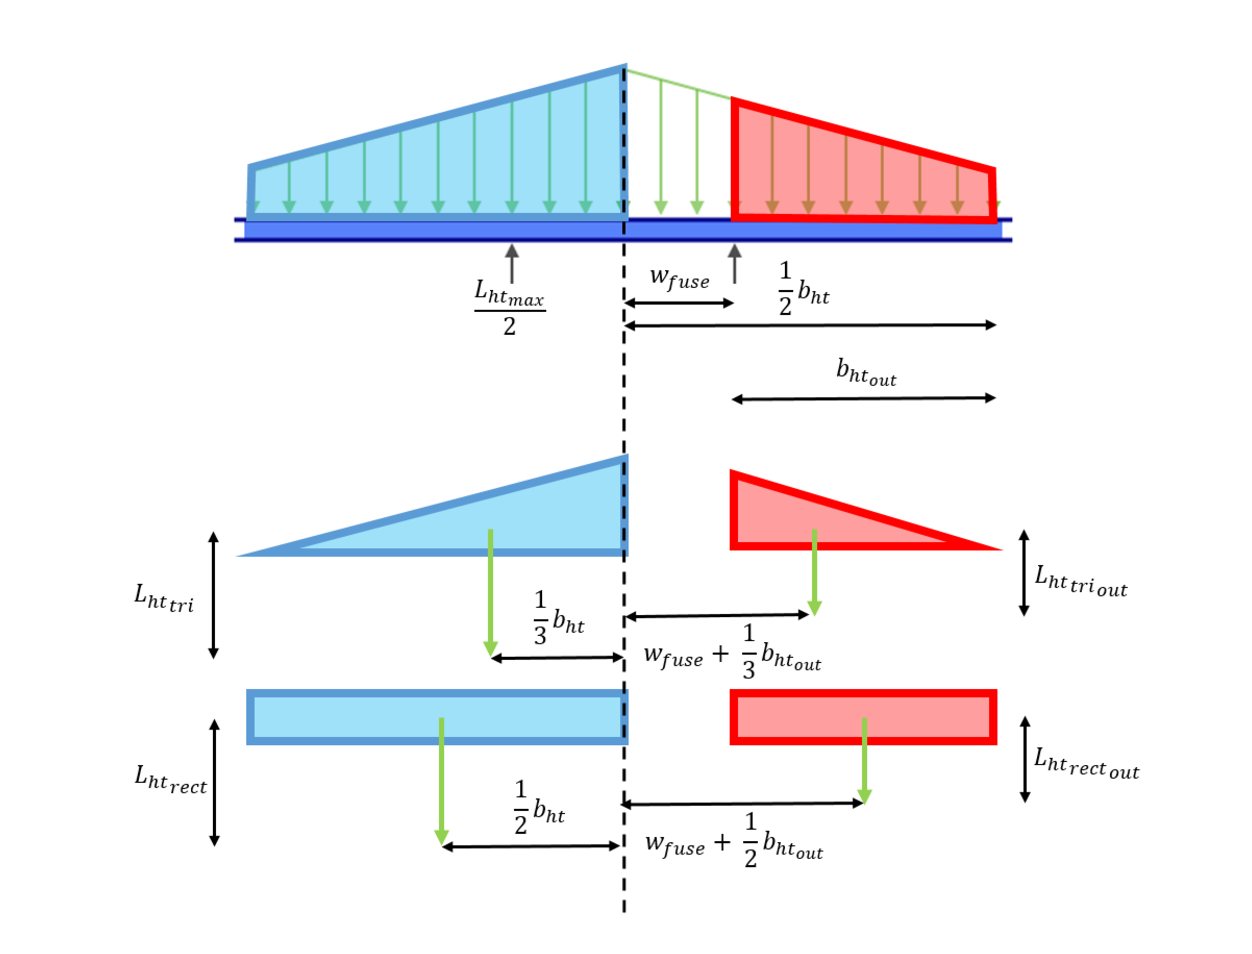
\includegraphics[width=.8\textwidth,natwidth=585,natheight=442]{HTFBD.eps}
\caption{Free body diagram of the forces on the horizontal tail. The distributed 
lift force, which is assumed to be proportional to local chord, is partitioned 
into triangular and rectangular components.}
\label{fig:HTFBD}
\end{figure}

Shear and moment diagrams are presented in Figures~\ref{fig:HTshear} and 
\ref{fig:HTmoment} respectively. The diagrams include both the distributed lift 
loads (green arrows in Figure \ref{fig:HTFBD}) and the point loads of imposed on 
the pin joints by the vertical tails.

\begin{figure}[!ht]
    \centering
    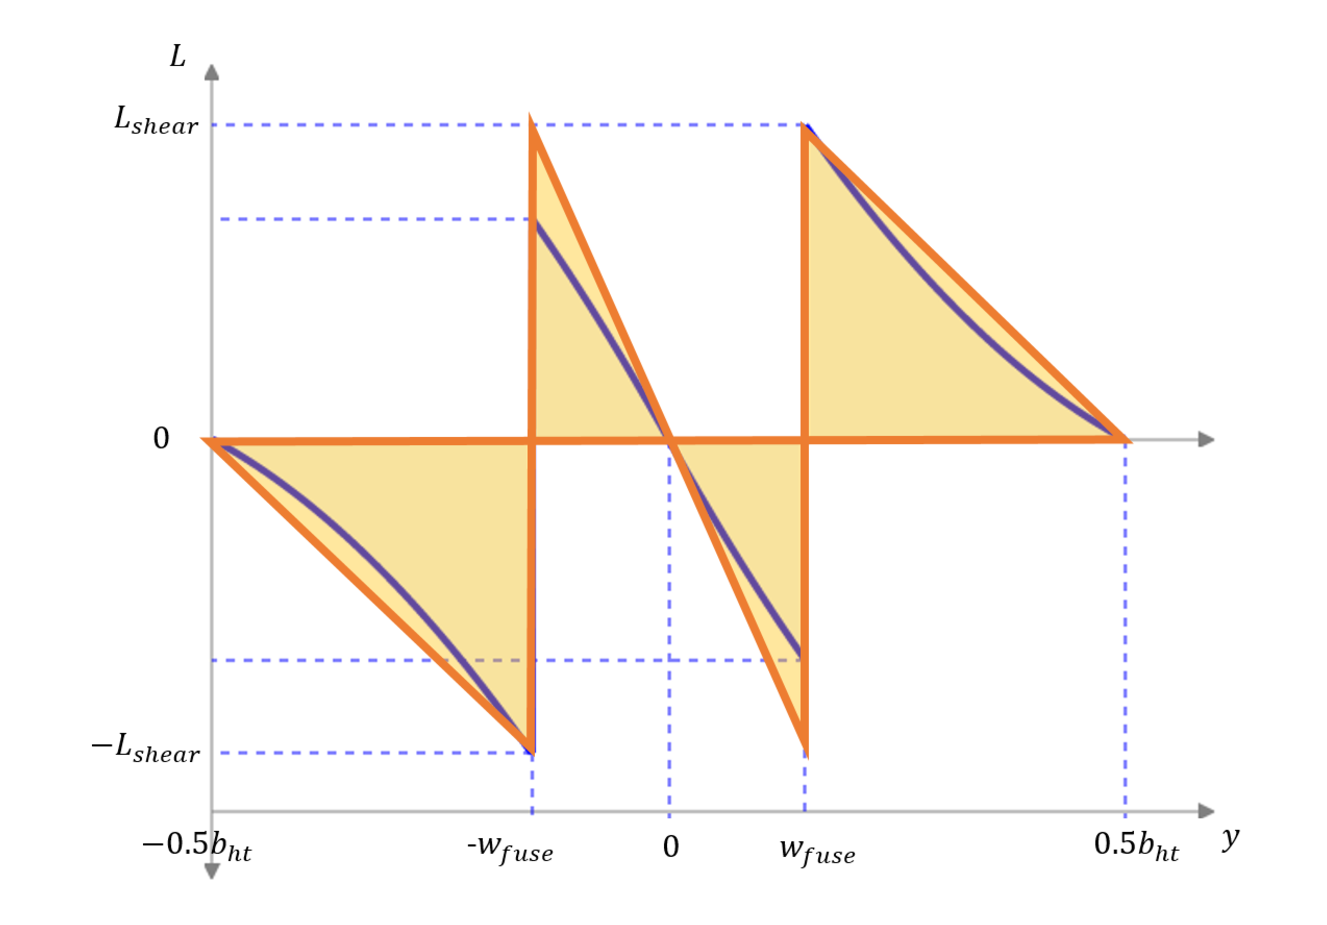
\includegraphics[width = 0.7\linewidth,natwidth=621,natheight=428]{HTshear.eps}
    \caption{Shear diagram of the pi-tail. The blue line shows the actual 
loading, while the yellow line with infill shows the assumed load distribution.}
    \label{fig:HTshear}
\end{figure}

\begin{figure}[!ht]
    \centering
    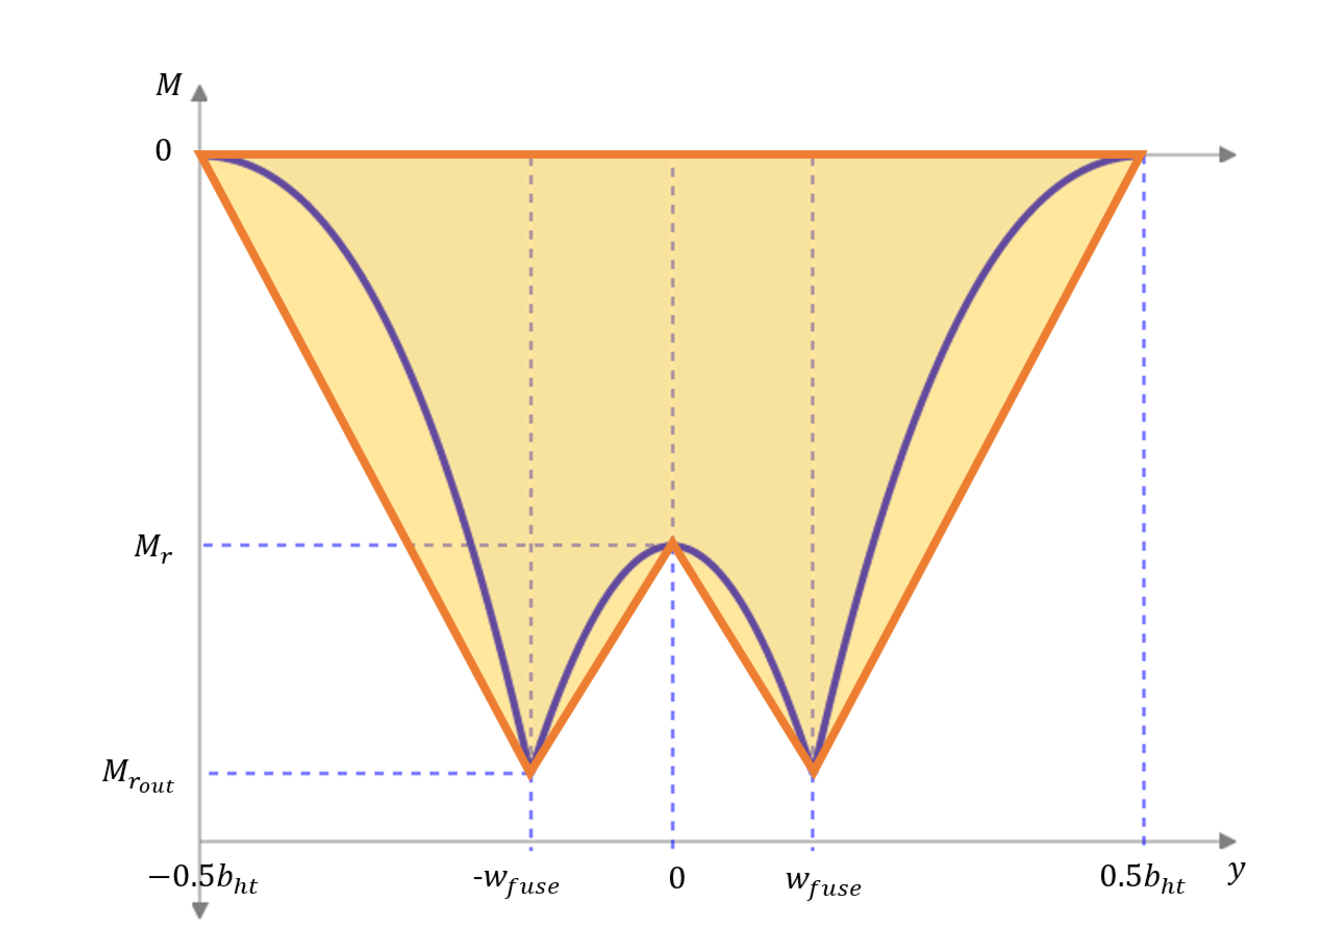
\includegraphics[width = 0.7\linewidth,natwidth=627,natheight=437]{HTmoment.eps}
    \caption{Moment diagram of the pi-tail. The blue line shows the actual 
loading, and the yellow line shows the assumed load distribution}
    \label{fig:HTmoment}
\end{figure}

After seeing these load distributions, an experienced \gls{GP} modeler would immediately think about linearization. 

\subsubsection{Assumptions}
\begin{enumerate}
    \item The lift per unit span is proportional to local chord.
    \item The horizontal tail has a constant taper ratio.
    \item The horizontal and vertical tail joint is a fuselage width away from 
the centerline of the aircraft. 
    \item The horizontal and vertical tail interface is a pin joint. Therefore, 
the joint does not exert a moment on the horizontal tail. 
    \label{item:pinjoint}
    \item The shear and moment distributions on the horizontal tail are 
linearized. 
\end{enumerate}

The pin-joint assumption ensures the vertical tail structural constraints do not 
need to be modified for the pi-tail configuration. 



\subsubsection{Horizontal Tail Terminology}
\begin{tabbing}
$I_{\rm{cap}}$ = non-dimensional spar cap area moment of inertia \\
$L_{\rm{ht}}$ = horizontal tail downforce \\
$L_{\rm{ht}_{\rm{max}}}$ = maximum horizontal tail downforce \\
$L_{\rm{ht}_{rect}}$ = rectangular horizontal tail load \\
$L_{\rm{ht}_{\rm{rect}_{\rm{out}}}}$ = rectangular horizontal tail load outboard\\
$L_{\rm{ht}_{\rm{tri}}}$ = triangular horizontal tail load \\
$L_{\rm{ht}_{tri_{\rm{out}}}}$ = triangular horizontal tail load outboard\\
$L_{\rm{shear}}$ = maximum shear load at pin-joint\\
$M_{\rm{r}}$ = moment per chord at horizontal tail root \\
$M_{\rm{r}_{\rm{out}}}$ = moment per chord at pin-joint\\
$N_{\rm{lift}}$ = horizontal tail loading multiplier \\
$S_{\rm{ht}}$ = horizontal tail area \\
$W_{\rm{cap}}$ = weight of spar caps \\
$W_{\rm{struct}}$ = horizontal tail wingbox weight \\
$W_{\rm{web}}$ = weight of shear web \\
$\lambda_{\rm{ht}}$ = horizontal tail taper ratio \\
$\nu$ = dummy variable = $(t^2 + t + 1)/(t+1)^2$ \\
$\pi_{\rm{M-fac}}$ = pi-tail bending structural factor \\
$\rho_{\rm{cap}}$ = density of spar cap material \\
$\rho_{\rm{web}}$ = density of shear web material \\
$\sigma_{max,shear}$ = allowable shear stress \\
$\sigma_{\rm{max}}$ = allowable tensile stress \\
$\tau_{\rm{ht}}$ = horizontal tail thickness/chord ratio \\
$b_{\rm{ht}}$ = horizontal tail span \\
$b_{\rm{ht}_{\rm{out}}}$ = horizontal tail outboard half-span\\
$c_{\rm{attach}}$ = horizontal tail chord at the pin-joint \\
$c_{\rm{root}_{\rm{ht}}}$ = horizontal tail root chord \\
$c_{\rm{tip}_{\rm{ht}}}$ = horizontal tail tip chord \\
$g$ = gravitational acceleration \\
$q_{\rm{ht}}$ = substituted variable = 1 + taper \\
$r_h$ = fractional wing thickness at spar web \\
$t_{\rm{cap}}$ = non-dim. spar cap thickness \\
$t_{\rm{web}}$ = non-dim. shear web thickness \\
$w$ = wingbox width-to-chord ratio \\
$w_{\textrm{fuse}}$ = fuselage half-width \\
\end{tabbing}

\subsubsection{Load Derivation}

$L_{\rm{ht}_{rect}}$ is defined to be half the lift generated by the `rectangular' 
section of the wing (the blue rectangle in Figure~\ref{fig:HTFBD}).

\begin{equation}
    L_{\rm{ht}_{rect}} \geq \frac{L_{\rm{ht}_{\rm{max}}} c_{\rm{tip}_{\rm{ht}}} b_{\rm{ht}}}{2 S_{\rm{ht}}}
\end{equation}

Similarly, $L_{\rm{ht}_{\rm{tri}}}$ is defined to be half the lift generated by the 
`triangular' section of the wing (the blue triangle in Figure~\ref{fig:HTFBD}).
 
\begin{equation}
     L_{\rm{ht}_{\rm{\rm{tri}}}} \geq \frac{L_{\rm{ht}_{\rm{max}}} (1 - \lambda_{\rm{ht}}) c_{\rm{root}_{\rm{ht}}} b_{\rm{ht}}}{4 
S_{\rm{ht}}}
\end{equation}
 
After defining the horizontal tail half-span outboard of the pin joint 
($b_{\rm{ht}_{\rm{out}}}$), the outboard components of the lift loads   can be computed 
with respect to $L_{\rm{ht}_{rect}}$ and $L_{\rm{ht}_{\rm{tri}}}$. The outboard loads are shown 
in red in Figure~\ref{fig:HTFBD}. 
 
 \begin{align}
     b_{\rm{ht}_{\rm{out}}} &\geq 0.5b_{\rm{ht}} - w_{\textrm{fuse}}\\
     L_{\rm{ht}_{tri_{\rm{out}}}} &\geq L_{\rm{ht}_{\rm{tri}}} \frac{b_{\rm{ht}_{\rm{out}}}}{(0.5b_{\rm{ht}})^2}\\
     L_{\rm{ht}_{\rm{rect}_{\rm{out}}}} &\geq L_{\rm{ht}_{rect}} \frac{b_{\rm{ht}_{\rm{out}}}}{0.5b_{\rm{ht}}}
 \end{align}
 
The horizontal-vertical tail pin joint is assumed to be exactly at $w_{\textrm{fuse}}$. 
This is a conservative estimate. In most pi-tail configurations the vertical 
tails are canted outwards. The local chord at the pin joint is constrained with 
the following monomial equality.
 
\begin{equation}
    c_{\rm{attach}} = \frac{b_{\rm{ht}} \lambda_{\rm{ht}} c_{\rm{root}_{\rm{ht}}}}{2 w_{\textrm{fuse}}}
\end{equation}
 
The maximum moment at the joint is determined by summing the bending moment 
contributions from loads outboard of the joint. 
\begin{equation}
M_{\rm{r}_{\rm{out}}} c_{\rm{attach}} \geq 
                    L_{\rm{ht}_{\rm{rect}_{\rm{out}}}} \frac{1}{2}b_{\rm{ht}_{\rm{out}}} + 
L_{\rm{ht}_{tri_{\rm{out}}}} \frac{1}{3}b_{\rm{ht}_{\rm{out}}},
\end{equation}
 
The maximum shear at the joint is the sum of the outboard shear loads. The 
maximum root moment is the sum of the bending loads from lift and the pin-joint 
load. 
 
\begin{align}
L_{\rm{shear}} &\geq L_{\rm{ht}_{\rm{rect}_{\rm{out}}}} + L_{\rm{ht}_{tri{\rm{out}}}}\\
M_{\rm{r}} c_{\rm{root}_{\rm{ht}}} &\geq L_{\rm{ht}_{\rm{rect}}} \frac{1}{4}b_{\rm{ht}} + L_{\rm{ht}_{\rm{\rm{tri}}}} 
\frac{1}{6}b_{\rm{ht}}  - \frac{1}{2}L_{\rm{ht}_{\rm{max}}} w_{\textrm{fuse}} 
\end{align}

Finally, the wingtip moment is set equal to zero with a signomial equality 
constraint.

\begin{equation}
    \frac{b_{\rm{ht}}}{4} L_{\rm{ht}_{\rm{rect}}} + \frac{b_{\rm{ht}}}{3} L_{\rm{ht}_{\rm{\rm{tri}}}} = b_{\rm{ht}_{\rm{out}}} 
\frac{L_{\rm{ht}_{\rm{max}}}}{2}
\end{equation}

\subsubsection{Structural Sizing}

Equations from \cite{gp_ac_design} for wing structural sizing were adapted using 
a linearization of the moment and shear load distributions from Appendix E2. The 
constraints can be applied to both conventional and pi-tails.

\begin{align}
    0.92 w\tau_{\rm{ht}} t_{\rm{cap}}^2 + I_{\rm{cap}} &\leq \frac{0.92^2}{2}w\tau_{\rm{ht}}^2t_{\rm{cap}}\\
    8 &\geq N_{\rm{lift}}M_{\rm{r}_{\rm{out}}}(\AR_{\rm{ht}})q_{\rm{ht}}^2\frac{\tau_{\rm{ht}}}{S_{\rm{ht}} I_{\rm{cap}}\sigma_{\rm{max}}}\\
    12 &\geq \frac{2L_{\rm{shear}} N_{\rm{lift}} q^2}{\tau_{\rm{ht}} S t_{\rm{web}} \sigma_{\rm{max-shear}}}
\end{align}

The changes to the model in \cite{gp_ac_design} are:
\begin{itemize}
    \item In the shear constraint replacing $L_{\rm{ht}_{\rm{max}}}$ with $2L_{\rm{shear}}$. 
This is done because the shear loads for the pi-tail are different than the 
maximum lift loads for the conventional tail. 
    \item Replacing $M_{\rm{r}}$ with $M_{\rm{r}_{\rm{out}}}$, the moment per unit chord at the 
pin joint. For a pi-tail, maximum bending loads occur at the pin joint.
    %, and along with the root moment per unit chord $M_{\rm{r}}$ can be used to give a 
    %conservative approximation for the mass of the horizontal tail. 
\end{itemize}

The linearization of the shear and bending load distributions simplifies the 
derivation of the structural web and cap weights. Shear web sizing relies on the 
assumption that the maximum shear ($L_{\rm{shear}}$) occurs at the pin-joint and the 
weight of the shear web of the pi-tail under $L_{\rm{shear}}$ is equal to the shear 
web weight of a conventional tail subjected to the the same maximum shear load 
at its root. This is a conservative approximation, the load distribution implied 
by this assumption (shown in yellow in Figure~\ref{fig:HTshear}) has a larger 
internal area than the actual load distribution. Intuitively, the $L_{\rm{shear}}$ 
for a pi-tail is strictly smaller than the $L_{\rm{shear}}$ a conventional tail of 
the same size and loading. The pi-tail more efficient in shear.

The cap weight of the pi-tail is determined by scaling the cap weight of a 
conventional tail with the same geometry as the pi-tail and a root moment of 
$M_{\rm{r}_{\rm{out}}} c_{\rm{attach}}$. The scaling factor, $\pi_{\rm{M-fac}}$, is the ratio of the 
total shaded bending moment area in Figure~\ref{fig:HTmoment} to the sum of the 
outboard shaded areas multiplied by the ratio of the outboard half-span to the 
total half-span.

\begin{equation}
    \pi_{\rm{M-fac}} \geq \left[\frac{\frac{1}{2}(M_{\rm{r}_{\rm{out}}} c_{\rm{attach}} +
    M_{\rm{r}} c_{\rm{root}_{\rm{ht}}}) w_{\textrm{fuse}}} {\frac{1}{2}M_{\rm{r}_{\rm{out}}} c_{\rm{attach}} 
b_{\rm{ht}_{\rm{out}}}} + 1.0\right]
    \frac{b_{\rm{ht}_{\rm{out}}}} {0.5b_{\rm{ht}}},
\end{equation}

Given the calculated loads and structural factors, the bending material and 
shear web weight can be calculated. 

\begin{align}
    W_{\rm{cap}} &\geq \frac{\pi_{\rm{M-fac}} 8 \rho_{\rm{cap}} g w t_{\rm{cap}} S_{\rm{ht}}^1.5 \nu}
    {3\AR_{\rm{ht}}^{0.5}}\\
    W_{\rm{web}} &\geq \frac{8 \rho_{\rm{web}} g r_h \tau_{\rm{ht}} t_{\rm{web}} S_{\rm{ht}}^{1.5} 
\nu}{3\AR_{\rm{ht}}^{0.5}}\\
    W_{\rm{struct}} &\geq W_{\rm{web}} + W_{\rm{cap}}
\end{align}

The value for $t_{\rm{cap}}$ is notional in the derivation above. Rather than being 
the spar cap thickness of a pi-tail, it is the spar cap thickness required for a 
conventional tail of the same geometry and a root moment  ($M_{\rm{r}_{\rm{out}}} 
c_{\rm{attach}}$) as a pi-tail. With a similar reasoning as for the shear loads, 
$\pi_{\rm{M-fac}} t_{\rm{cap}}$ for a pi-tail is strictly smaller than the $t_{\rm{cap}}$ for a 
conventional tail of the same geometry and loading, making the pi-tail more 
efficient in bending than a traditional tail. 